%----------------------------------------------------------------------------------------
%	METODE
%----------------------------------------------------------------------------------------
\section*{METODE PENELITIAN}

Penelitian yang dilakukan terbagi menjadi beberapa tahapan proses. Gambar \ref{fig:metodepenelitian} menunjukan tahapan proses tersebut.

\begin{figure}[h!]
	\centering
	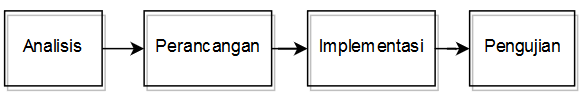
\includegraphics[width=220pt]{gambar/metode_penelitian}
	\caption{Metode Penelitian}
	\label{fig:metodepenelitian}
\end{figure}

\subsection*{Analisis}

Pada tahap ini dimulai dari membaca literatur terkait dan mendefinisikan kebutuhan dari aplikasi yang akan dibangun. Selain itu, pada tahapan ini juga dilakukan pengumpulan berapa contoh program yang akan digunakan dalam penelitian. Contoh program yang digunakan dalam penelitian ini didapatkan dari penelitian yang dilakukan oleh \citeauthor{HERMADI2015} (\cite*{HERMADI2015}).  

\subsection*{Perancangan}
Pada tahap ini ditentukan bagaimana perangkat lunak akan dibangun. Ilustrasi arsitektur sistem dapat dilihat pada Gambar \ref{fig:struktur}.
\begin{figure}[h!]
	\centering
	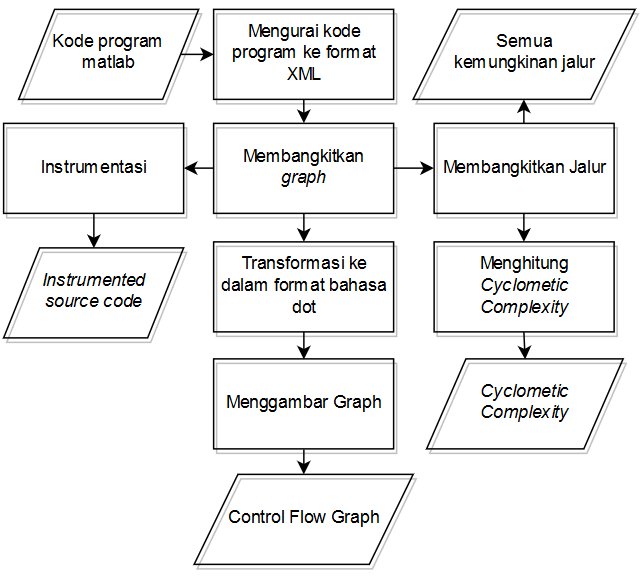
\includegraphics[width=230pt]{gambar/struktur}
	\caption{Arsitektur Sistem}
	\label{fig:struktur}
\end{figure}

\subsubsection*{Kode Program}
Kode program matlab akan dibaca sebagai inputan. Matlab merupakan singkatan dari MATrix LABoratory. Seperti bahasa pemrograman lainnya, matlab memiliki beberapa sruktur kontrol. Struktur kontrol adalah perintah dalam bahasa pemrograman yang digunakan dalam pengambilan keputusan. Matlab memiliki empat struktur kontrol, yaitu IF-ELSE-END, SWITCH-CASE, FOR, dan WHILE (\cite{HOUCQUE2005}). 

\subsubsection*{Mengurai Kode Progam ke Format XML}
Penguraian kode program matlab dilakukan dengan menggunakan library  MATLAB-PARSER. Ketika terdapat kesalahan pada kode program, library  ini akan mengembalikan pesan \textit{error}. Lalu kode program tersebut diurai menjadi file dengan format XML menggunakan \textit{library} MATLAB-PARSER yang dibuat oleh  \citeauthor{SUFFOSPARSER2005} (\cite*{SUFFOSPARSER2005}). 

\textit{Extensible Markup Language} (XML) adalah bahasa yang dapat mendeskripsikan sebuah dokumen. XML memiliki banyak bagian yang tidak memiliki struktur yang pasti. XML terdiri atas dua bagian utama, yaitu elemen dan atribut. Elemen yang dapat disebut sebagai \textit{node} merupakan bagian penting yang dapat menggambarkan struktur dari XML. Sedangkan atribut merupakan bagian yang dapat digunakan sebegai informasi tambahan dari setiap elemen  (\cite{HARTWELL2017}). 

\subsubsection*{Membangkitkan \textit{Graph}}
Setiap elemen dalam file XML tersebut akan ditelusuri satu persatu yang termasuk struktur kontrol di dalam bahasa matlab. Sehingga terbentuklah sebuah objek \textit{graph} yang terdiri dari sekumpulan \textit{node} dan \textit{edge}. 

Salah satu cara untuk membaca dan menulis dokumen XML pada \textit{framework} .NET dan C\# yaitu dengan menggunakan kelas XMLDocument yang terdapat dalam\textit{ namespace System.XML}. Setiap elemen XML yang merupakan struktur kontrol pada program akan menjadi \textit{node} baru di dalam kelas \textit{graph}. Setiap \textit{node} berisi informasi nomor baris dan kolom yang akan digunakan untuk melakukan instrumentasi.

\subsubsection*{Membangkitkan Jalur}
\textit{Basis path testing} merupakan salah satu metode pengujian struktural yang menggunakan \textit{source code} dari program untuk menemukan semua jalur yang mungkin dapat dilalui program dan dapat digunakan untuk merancang data uji. Metode ini memastikan semua kemungkinan jalur dijalankan setidaknya satu kali (\cite{BASU2015}). 

Metode ini terbagi menjadi 4 tahapan, yaitu:
\begin{enumerate}[noitemsep] 
	\item Menggambarkan jalur dalam bentuk \textit{ Control Flow Graph} (CFG)
	\item Menghitung \textit{cyclomatic complexity}
	\item Memilih satu set jalur dasar
	\item Membangkitkan data uji untuk setiap jalur dasar
\end{enumerate}


\subsubsection*{Transformasi ke Dalam Format Bahasa Dot}
\textit{Graph} yang sudah terbentuk akan ditransformasikan ke dalam bentuk format bahasa permrograman dot. Bahasa dot adalah bahasa yang digunakan untuk mengambar \textit{graph} berarah. Bahasa ini dapat mendeskripsikan 3 macam objek, yaitu \textit{graph}, \textit{nodes}, dan \textit{edges} (\cite{GANSNER2015}).

\subsubsection*{Memvisualisasi \textit{Graph} dalam bentuk CFG}
\textit{Control Flow Graph }(CFG) adalah graph berarah yang merepresentasikan aliran dari sebuah program. Setiap CFG terdiri dari \textit{nodes} dan \textit{edges}. \textit{Nodes} merepresentasikan \textit{statement} atau \textit{expressions}. Sedangkan \textit{edges} merepresentasikan transfer kontrol antar \textit{nodes} (\cite{MCCABE}). Notasi dari CFG dapat dilihat pada Gambar \ref{fig:cfg}.
\begin{figure}[h]
	\centering
	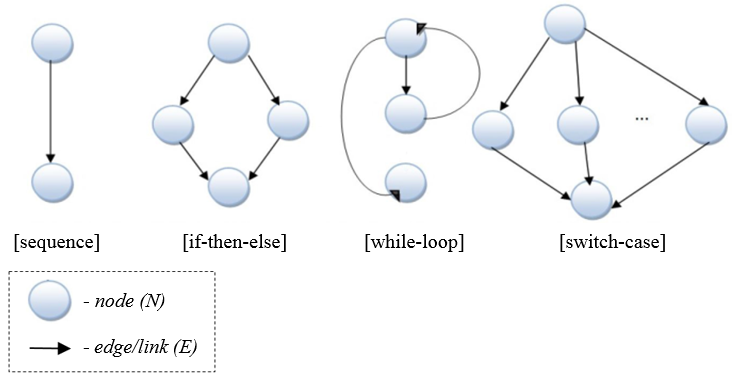
\includegraphics[width=0.9\linewidth]{gambar/CFG}
	\caption{Notasi Control Flow Graph (CFG)}
	\label{fig:cfg}
\end{figure}
Setelah file dengan format bahasa dot terbentuk, CFG akan divisualisasikan dengan menggunakan library Graphviz. Graphviz merupakan perangkat lunak open source untuk visualisasi grafik. Graphviz memiliki banyak fitur berguna untuk menggambar diagram yang konkret karena terdapat pilihan warna, font, tata letak, jenis garis, dan bentuk (\cite{ELLSONGRAPHVIZ2003}).
\subsubsection*{Menghitung \textit{Cyclometic Complexity}}

\textit{Cyclomatic complexity} merupakan suatu sistem pengukuran yang ditemukan oleh \citeauthor{MCCABE} untuk menentukan banyaknya \textit{independent path} dan menunjukan tingkat kompleksitas dari suatu program. \textit{Independent path} adalah jalur yang melintas dalam program yang sekurang-kurangnya terdapat kondisi baru. Perhitungan \textit{Cyclomatic Complexity} dapat dilihat pada persamaan berikut:
\[V(G)=E-N+2\]

Dimana, E menunjukkan jumlah \textit{edges} dan N menunjukkan jumlah \textit{nodes}.

\subsubsection*{Instrumentasi}
Setelah jalur terbentuk, dilakukan juga proses instrumentasi. Instrumentasi merupakan sebuah proses menyisipkan sebuah penanda (tag) di awal atau di akhir setiap blok kode seperti awal setiap perintah, sebelum atau sesudah kondisi terpenuhi atau tidak. Dalam pengujian path testing, penanda ini dapat digunakan untuk memonitor jalur yang dilalui program ketika dijalankan dengan masukan data uji tertentu (\cite{IRH2014}). 

Instrumentasi dilakukan dengan cara menambahkan dulu variabel keluaran bernama \textit{traversedPath}. Variabel in digunakan untuk menyimpan informasi node mana saja yang dilalui ketika diberikan inputan dengan nilai tertentu. Lalu setiap sebelum dan sesudah \textit{node} percabangan, dilakukan penyisipan kode program berupa perintah untuk memasukkan nilai \textit{node} yang dilalui. Sehingga ketika program tersebut dijalankan, akan menghasilkan keluaran tambahan bernama \textit{traversedPath}. 

\subsection*{Implementasi}

Tahapan ini adalah melakukan implementasi dari tahap sebelumnya ke dalam bentuk aplikasi web. Aplikasi ini akan dibangun dengan menggunakan bahasa pemrograman C\# dan menggunakan IDE Microsoft Visual Studio Ultimate 2013. 

Setelah file dengan format bahasa dot terbentuk, CFG divisualisasikan dengan menggunakan \textit{library} Graphviz.Net. Graphviz.Net adalah pembungkus C\# untuk generator grafik Graphviz yang dibuat oleh \citeauthor{DIXONGRAPHVIZ2013} (\cite*{DIXONGRAPHVIZ2013}). Keluaran yang dikembalikan ketika mengeksekusi Graphviz.Net berbentuk \textit{byte} dalam \textit{array} sehingga dapat diolah kembali sesuai dengan kebutuhan. Graphviz merupakan library yang dapat digunakan untuk menvisualisasi jalur ke dalam bentuk graph berarah (\cite{GANSNER2015}). 


\subsection*{Testing}

Tahapan ini adalah melakukan evaluasi dari tahapan implementasi. Evaluasi dibagi menjadi dua bagian, yaitu uji validasi dan uji efisiensi. Uji validasi dilakukan dengan cara membandingkan hasil yang ada pada penelitian sebelumnya dengan hasil yang dikeluarkan oleh aplikasi. Pada penelitian sebelumnya, \textit{graph} yang dibangun adalah \textit{graph} yang hanya menggambarkan notasi percabangan. Agar dapat dibandingkan dengan hasil yang dikeluarkan oleh aplikasi, \textit{graph} yang ada pada penelitian sebelumnya direpresentasikan ke dalam bentuk \textit{adjacency list} terlebih dahulu secara manual.

Uji efisiensi dilakukan dengan membandingkan waktu eksekusi yang dilaukan secara manual dengan waktu eksekusi oleh aplikasi. Pengujian manual akan dilakukan dengan meminta satu atau dua orang yang sudah memiliki pengalaman dalam pemrograman sebagai sampel  untuk melihat berapa lama waktu yang dibutuhkan untuk membangkitkan CFG, membangkitkan semua kemungkinan jalur,  menghitung \textit{cyclomatic complexity}, dan melakukan instrumentasi.
